\documentclass[hyperref={pdfpagelabels=false}]{beamer}
\usepackage{lmodern}
\usepackage[T1]{fontenc}
\usetheme{Frankfurt}
\usecolortheme{beaver}
\usepackage{graphicx}
\usepackage{apacite}
\bibliographystyle{apacite}


\title{The link between football and domestic abuse in England: evidence from the West Midlands}  
\author{Anna Trendl} 
\date{\today} 
\begin{document}
\begin{frame}
\titlepage
\end{frame} 


\section{Domestic abuse in England} 
\begin{frame}
\frametitle{Domestic abuse in England} 
\begin{itemize}
\item ``any incident of controlling, coercive or threatening behaviour, violence or abuse (psychological, physical, sexual, financial or emotional) between those aged 16 or over who are or have been intimate partners or family members'' \cite{cps}
\item almost two million people (0.695 million men and 1.3 million women) have reported to have experienced some form of domestic abuse in England and Wales in the year ending March, 2018 \cite{ONS}
\item the estimated economic cost of domestic abuse in the year ending March, 2017 was \pounds 66 billion \cite{costs}
\end{itemize}
\end{frame}



\begin{frame}
\frametitle{The link between football and domestic abuse in England}
\begin{center}
\begin{figure}
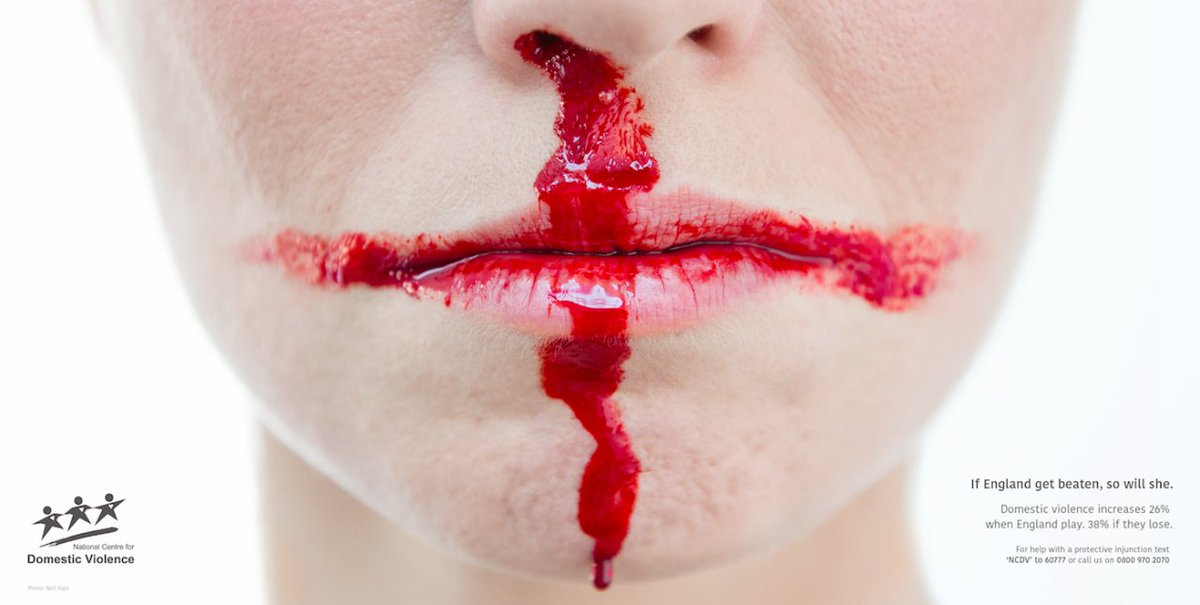
\includegraphics[scale=0.15]{domesticviolence.jpg}
\end{figure}
\end{center}
\begin{itemize}
\item ``If England get beaten, so will she. Domestic violence increases 26\% when England play, 38\% if they lose.''
%\item \citeNP{Kirby2014}: \textit{Can the FIFA World Cup
%Football (Soccer) Tournament Be Associated with an Increase in Domestic
%Abuse?}

\item \citeNP{Kirby2014}: daily number of domestic abuse (IPV) cases reported to the Lancashire Constabulary during the 2002, 2006 and 2010 World Cups 
\item Does the pattern replicate using data from a different time period, and geographical area within England? What is the role of alcohol in this relationship?
\end{itemize}
\end{frame}

%\begin{frame}
%\frametitle{The link between football and domestic abuse in England}
%\begin{itemize}
%\item Kirby et al., 2014: daily number of domestic abuse (IPV) cases reported to the Lancashire Constabulary (population of 1.4 million) during the 2002, 2006 and 2010 World Cups 
%\item Does the pattern replicate using data from a different time period, and geographical area within England? 
%\item What is the role of alcohol in this relationship? 
%\end{itemize} 
%\end{frame}

\section{Data} 

\begin{frame}
\frametitle{Data}
\begin{itemize}
\item All crimes and incidents recorded by the West Midlands Police (WMP) in the period between 2010 and 2018 
\item 31\% of all cases recorded are domestic abuse related, average daily rate of reported domestic abuse cases is 3.11 per 100,000 individuals
\item exact time of incident, age, gender of victim and perpetrator, alcohol involvement in the case
\item England participated in 5 international football tournaments within this period (3 World Cups, 2 Euro Cups)
\end{itemize} 
\end{frame}

\section{Methodology} 

\begin{frame}
\frametitle{Methodological Approach}
%    \begin{equation}
%            ln(No.cases_{i}) = g(Type.of.day_{i}, Alcohol_{i}, Time.Controls_{i})
%    \end{equation}
\begin{itemize}
\item Outcome variable: daily number of reported domestic abuse cases
\item Explanatory variables: 
 \begin{itemize}
\item Type.of.day: Nonmatch day (2867), Tournament on (106), England win (8), lose (8) or draw (6), Day after England (22)
\item Alcohol-involvement in the cases (Yes/No)
\item Time.Controls: year, month, day of the week, Christmas, NYE
\end{itemize} 
\end{itemize} 
\end{frame}

\section{Results} 
\begin{frame}
\frametitle{Results I - Model specifications}
\begin{center}
\begin{figure}
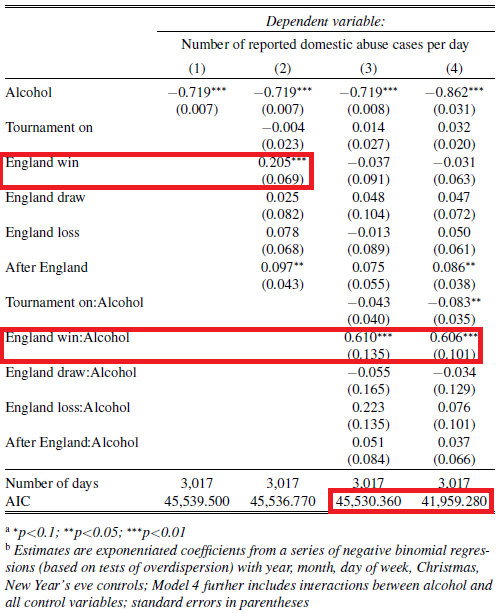
\includegraphics[scale=0.55]{result1.png}
\end{figure}
\end{center}
\end{frame}

\begin{frame}
\frametitle{Results II - Three hour analysis}
\begin{center}
\begin{figure}
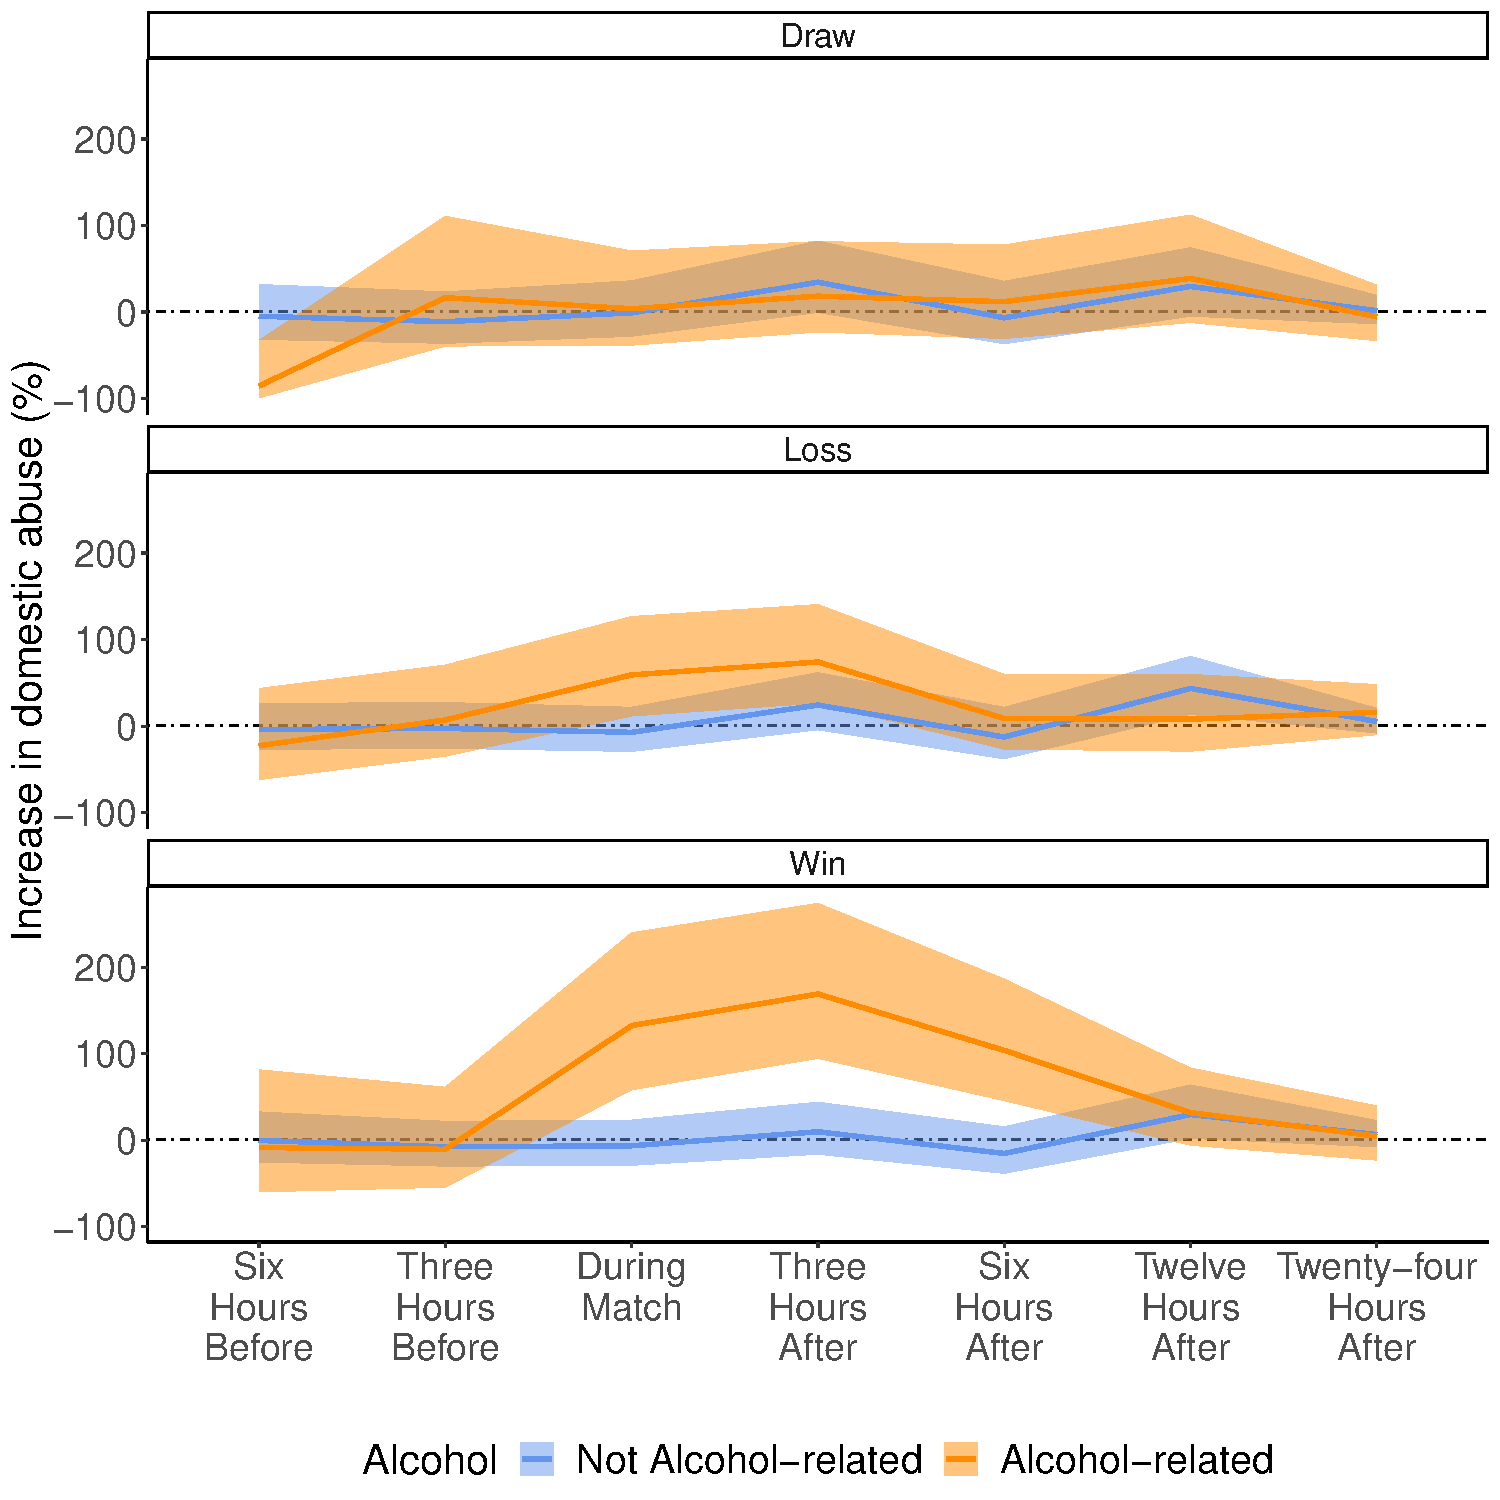
\includegraphics[scale=0.3]{Threehours.pdf}
\end{figure}
\end{center}
\end{frame}



\begin{frame}
\frametitle{Results III - Gender subgroups, Rugby, Other offences}
\begin{center}
\begin{figure}
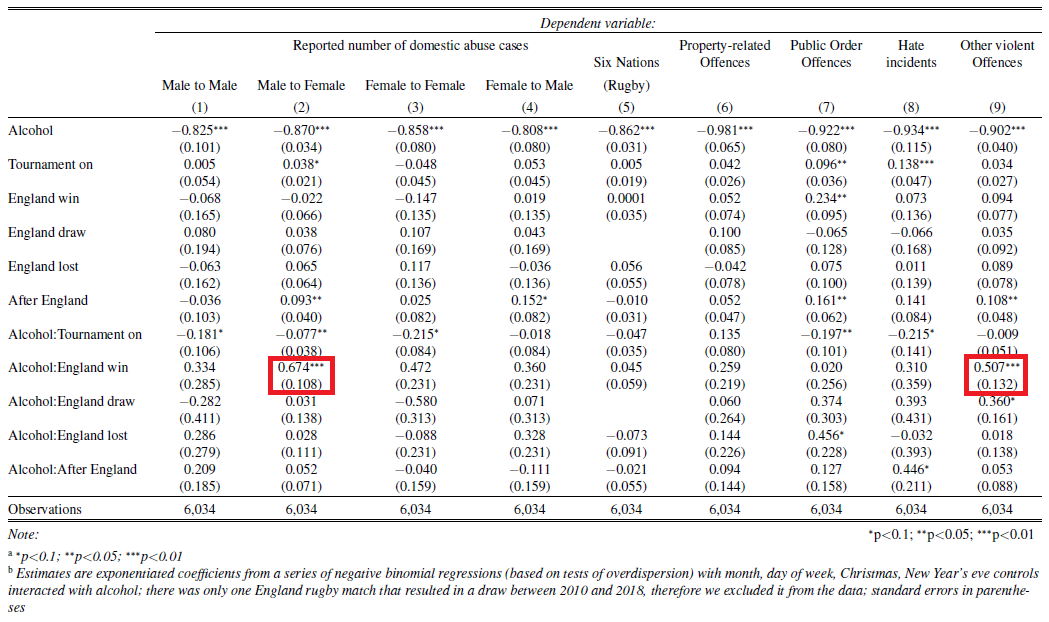
\includegraphics[scale=0.5]{result2.png}
\end{figure}
\end{center}
\end{frame}


\begin{frame}
\begin{center}
\begin{figure}
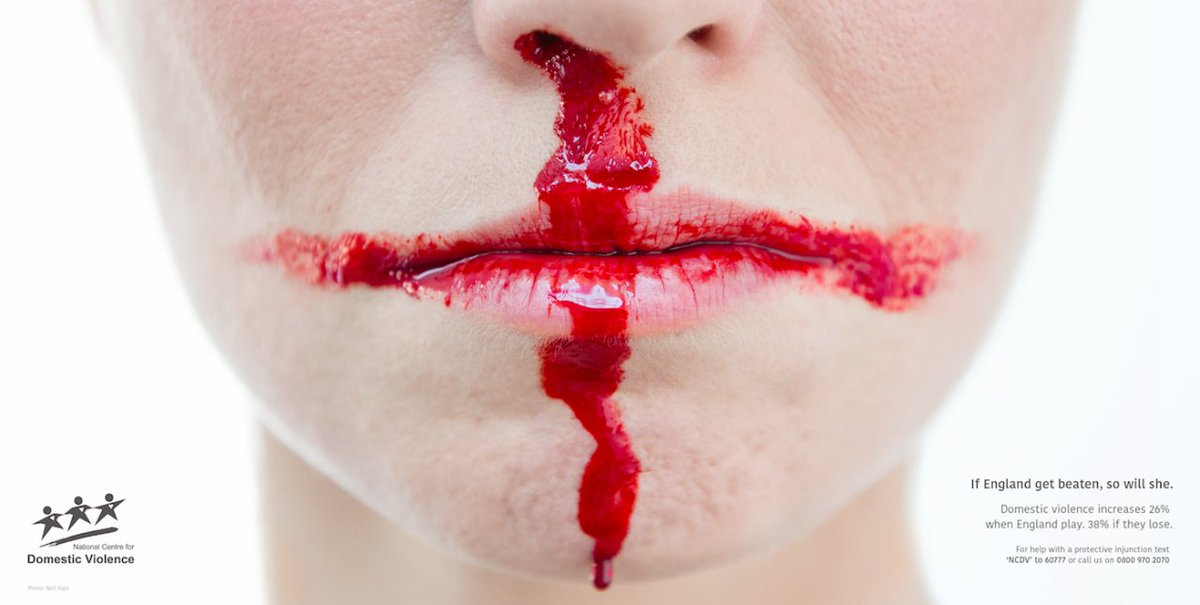
\includegraphics[scale=0.15]{domesticviolence.jpg}
\end{figure}
 ``If England get beaten, so will she. Domestic violence increases 26\% when England play, 38\% if they lose.''
\end{center}
\end{frame}

\begin{frame}
\frametitle{Results IV - Kirby et al. (2014) replication}
\begin{center}
\begin{figure}
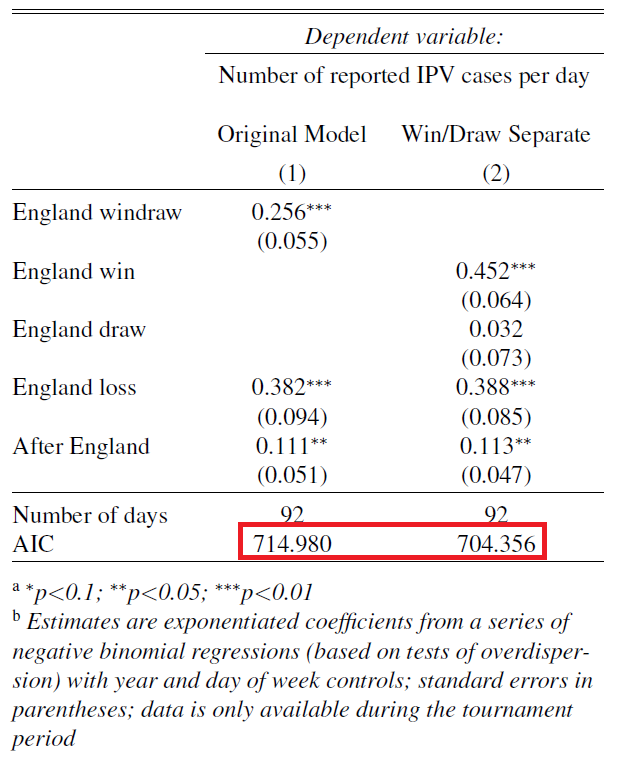
\includegraphics[scale=0.45]{result3.png}
\end{figure}
\end{center}
\end{frame}

\begin{frame}
\frametitle{Results IV - Robustness checks}
\begin{center}
\begin{figure}
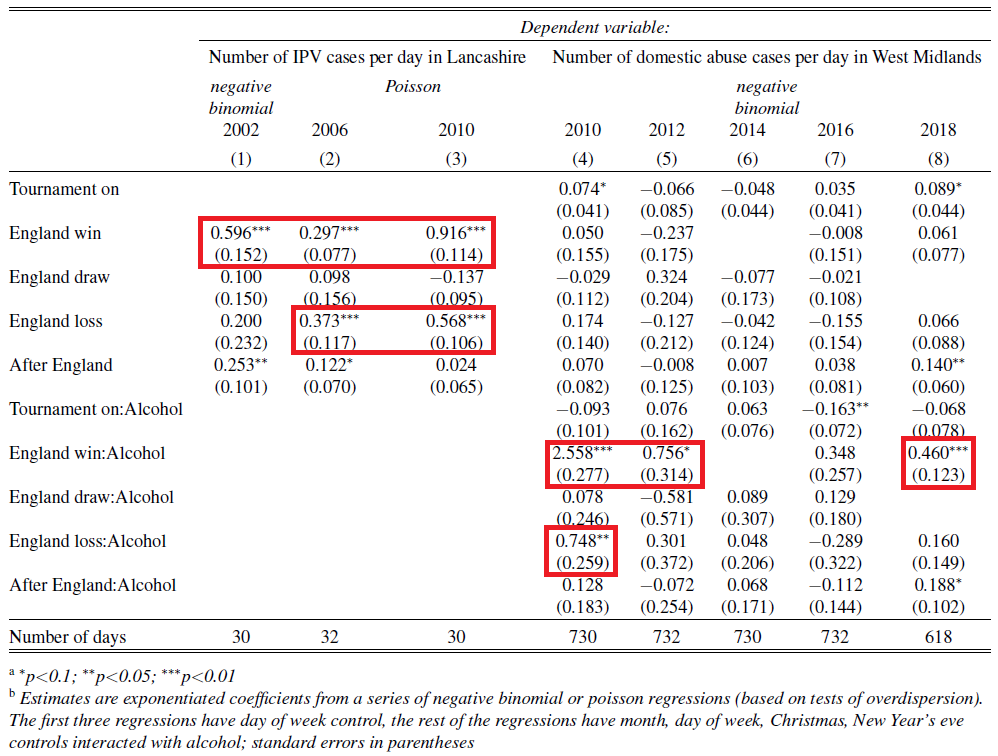
\includegraphics[scale=0.45]{result4.png}
\end{figure}
\end{center}
\end{frame}

\begin{frame}
\frametitle{Results IV - Robustness checks}
\begin{center}
\begin{figure}
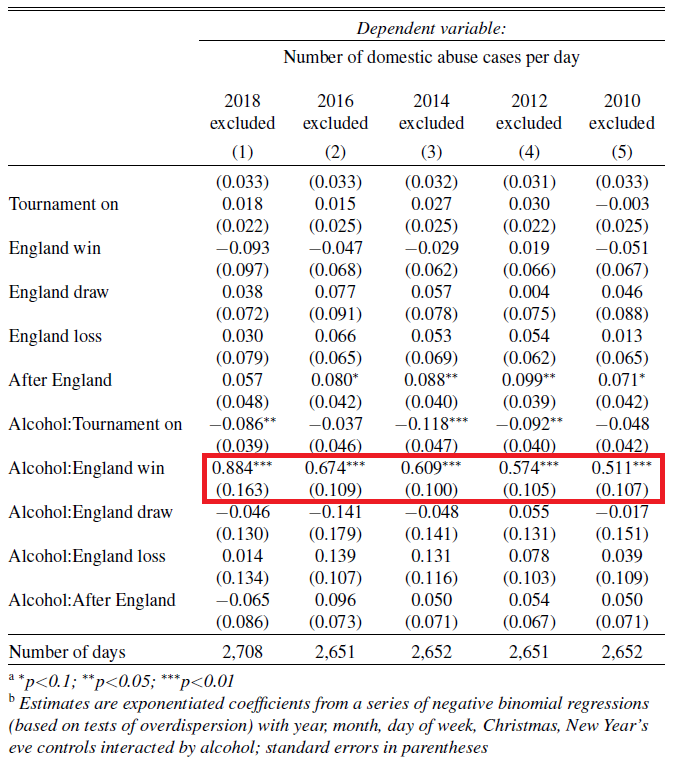
\includegraphics[scale=0.45]{result5.png}
\end{figure}
\end{center}
\end{frame}

\section{Conclusion}

\begin{frame}
\frametitle{Summary}
\begin{itemize}
\item All crimes and incidents recorded by the West Midlands Police between 2010-2018
\item Alcohol-related domestic abuse increases by 61\% following an England victory, its temporal dynamics suggests a causal link, non-alcohol related abuse is unaffected
\item The effect is specific to male to female abuse and football 
\item The win effect is consistent across different time periods and geographical areas

\end{itemize}
\end{frame}


\begin{frame}[shrink=20]{}
\frametitle{References}

\bibliography{presrefs}
\end{frame}

\section{Appendix}

\begin{frame}
\frametitle{}
\begin{center}
\huge Appendix
\end{center}
\end{frame}


\begin{frame}
\frametitle{Other violence - Gender subgroups}
\begin{center}
\begin{figure}
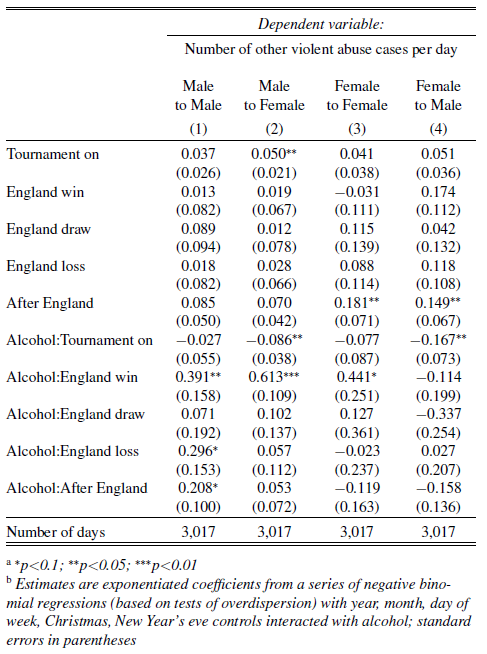
\includegraphics[scale=0.45]{append1.png}
\end{figure}
\end{center}
\end{frame}

\begin{frame}
\frametitle{Characteristics I}
\begin{center}
\begin{figure}
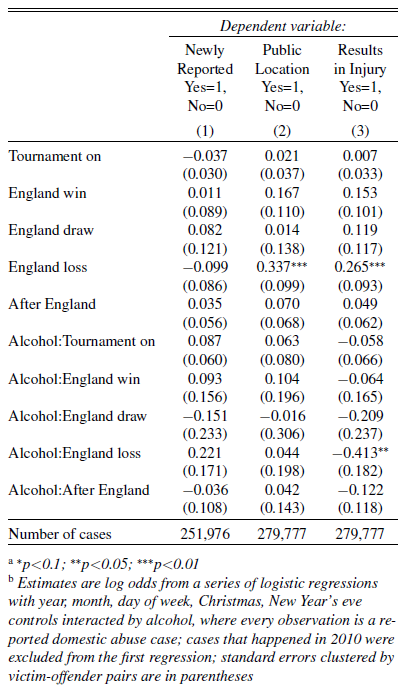
\includegraphics[scale=0.45]{append2.png}
\end{figure}
\end{center}
\end{frame}

\begin{frame}
\frametitle{Characteristics II}
\begin{center}
\begin{figure}
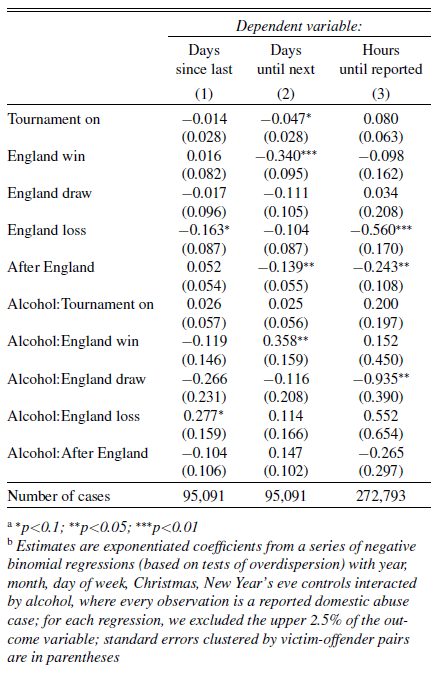
\includegraphics[scale=0.45]{append3.png}
\end{figure}
\end{center}
\end{frame}

\begin{frame}
\frametitle{Characteristics III}
\begin{center}
\begin{figure}
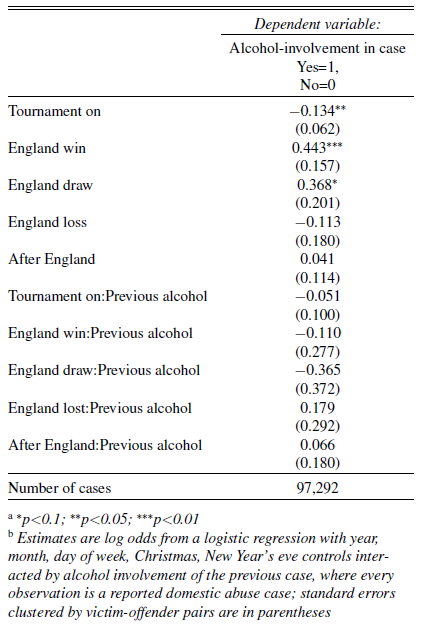
\includegraphics[scale=0.45]{append4.png}
\end{figure}
\end{center}
\end{frame}


\end{document}
